% !TEX root = main.tex
\pdfoptionpdfminorversion=7
\documentclass[12pt]{article}
\usepackage[utf8]{inputenc}
% Permite usar guiones bajos sin entrar accidentalmente en modo matemático.
% \usepackage[strings]{underscore}

% 1. Desactiva los shorthands para evitar el conflicto entre babel-spanish y biblatex-apa
\usepackage[spanish, shorthands=off]{babel}

% 2. Requerido por biblatex-apa para gestionar citas contextuales y comillas en español
\usepackage{csquotes}

% 3. Estilo de bibliografía APA 7ma edición
\usepackage[style=apa]{biblatex}

% Carga el paquete necesario para insertar imágenes (PDF, PNG, JPG)
\usepackage{graphicx}

% Le enseña a LaTeX a buscar imágenes un nivel arriba
\graphicspath{{../images/}}

% Ruta al archivo de bibliografía desde la raíz del proyecto
\addbibresource{../refs/references.bib} 

\usepackage{amsmath} % Permite usar \text{} dentro de fórmulas matemáticas

\begin{document}

% Inclusión modular de capítulos
\begin{titlepage}
    \centering
    \vspace*{0.5cm}

    % Logo Universitario
    
\includegraphics[width=3.5cm]{../images/logo-sociales.png}
    \vspace{0.8cm}

    {\Large\bfseries Universidad de Chile}\\[0.2cm]
    {\large Facultad de Ciencias Sociales}\\[2.5cm]

    {\huge\bfseries Ingresos y Costo de Vida en el Cono Sur}\\[0.5cm]
    {\large Evidencia de Chile, Brasil y Argentina (2015--2025)}\\[3cm]

    \textbf{Autor:} Vicente Rojas Murúa\\[0.3cm]
    \textbf{Profesor Guía:} Dr. Gonzalo Durán Sanhueza

    \vfill

    {\large Santiago, Chile}\\[0.2cm]
    {\large 2026}\\[0.2cm]
    {\large (avance al 28.09.2026)}
\end{titlepage}
\section{Introducción}

Este trabajo\footnote[1]{Se utilizan los Lineamientos FACSO para la elaboración de este proyecto, donde los proyectos "(...) pueden seguir un formato de investigación empírica, discusión teórica, o intervención político social. El desarrollo del Seminario de Grado va a depender del tipo de enfoque que la o el estudiante decida adoptar. No obstante, hay elementos comunes que deberán ser abordados a lo largo de las secciones del Seminario de Grado. Estos incluyen antecedentes problematización, objetivos, perspectiva teórica y metodológica. El orden en que se presentan estos elementos puede variar (por ejemplo, la problematización puede situarse después de los antecedentes y perspectiva teórica)."} examina comparativamente la relación entre el ingreso familiar y el costo de vida en Chile, Brasil y Argentina durante el decenio 2015–2025. Este período se ha caracterizado por complejas transformaciones macroeconómicas, presiones inflacionarias disímiles o diferentes y reajustes estructurales en el mercado de trabajo regional \parencite{cepalPanoramaSocialAmerica2025}. Diversos estudios han evidenciado que la inflación no impacta de manera homogénea a la población, manifestando brechas diferenciadas según el nivel socioeconómico de los hogares \parencite{Adam2025, doValleGomesdaSilva2026} y forzando la adopción de estrategias de consumo de subsistencia ante el encarecimiento de bienes básicos \parencite{Nessieretal2026}. Asimismo, la dinámica entre la inflación de precios y la evolución salarial \parencite{Malheretal2026}, condicionada por la efectividad del salario mínimo \parencite{GindlingRonconi2025, MaurizioVazquez2016} y la heterogeneidad de los ingresos laborales \parencite{DuranKremerman2024, INE2024}, resulta determinante para evaluar las alteraciones en el poder adquisitivo y el grado de vulnerabilidad socioeconómica familiar.

A través de una perspectiva comparada y multidisciplinar, la investigación indaga en las mediaciones entre estas variaciones macroeconómicas y las condiciones materiales de vida de las familias en cada caso de estudio. 

Para ello, la propuesta se articula en un doble pilar analítico: por un lado, un cuerpo de antecedentes empíricos enfocado en la distribución del ingreso \parencite{ResumenResultadosCASEN2023}, la efectividad estabilizadora de las transferencias condicionadas y la protección social \parencite{Stampinietal2025, Carrere2026}, así como el rol de las instituciones laborales y el poder sindical \parencite{BarreraInsuaNoguera2026, DuranS2026}; por otro lado, un marco teórico que integra la economía política del trabajo y la acumulación de capital \parencite{DuranSilva2022, MarxElCapital2008} con los enfoques contemporáneos sobre estratificación social y reproducción del bienestar en América Latina \parencite{cepalPanoramaSocialAmerica2025, CostaRibeiroCarcalhaes2024}.
\section{Antecedentes Empíricos}

La literatura sobre las dinámicas distributivas, el costo de vida y los mercados laborales en América Latina evidencia un cuerpo amplio de investigaciones aplicadas. Para abordar la relación entre los ingresos de los hogares y el costo de vida en Chile, Brasil y Argentina, la evidencia empírica seleccionada se sistematiza en cinco ejes analíticos fundamentales: i) estructura laboral, política salarial e institucionalidad del trabajo; ii) dinámica inflacionaria, formación de precios y costo de vida; iii) protección social, transferencias monetarias y mitigación de la pobreza; iv) concentración de ingresos, riqueza y brechas interseccionales (raza y género); y v) movilidad social, estratificación y percepciones de la desigualdad. La definición de estos ejes se fundamenta en la revisión de la literatura especializada y su proceso de sistematización detallado a continuación.

\subsection{Estrategia de Búsqueda, Limitaciones y Fuentes Institucionales}

Para fundamentar el estado del arte y garantizar un marco de antecedentes transparente, exhaustivo y replicable, se diseñó una estrategia de búsqueda bibliográfica híbrida basada en los lineamientos del protocolo PRISMA 2020\footnote[2]{PRISMA significa \textit{Preferred Reporting Items for Systematic Reviews and Meta-Analyses} (Elementos de información preferidos para revisiones sistemáticas y metaanálisis). La versión 2020 reemplaza a la antigua guía de 2009 para adaptarse a los nuevos avances metodológicos en la investigación. https://www.sciencedirect.com/science/article/pii/S0300893221002748} (Figura~\ref{fig:prisma-flowchart}) se profundizan en el \textbf{Anexo 1}. Esta estrategia articuló la captura sistemática de literatura científica de alto impacto en la colección principal de \textit{Web of Science} (WoS) con búsquedas complementarias en repositorios regionales de acceso abierto (\textit{SciELO}, \textit{Redalyc}, \textit{Dialnet} y \textit{Google Académico}) en español y portugués, sumada a la incorporación estructurada de literatura gris institucional.\footnote{Se entiende por literatura gris aquel conjunto de documentos y publicaciones técnicas de carácter público u oficial —como informes de organismos multilaterales, boletines estadísticos, documentos de trabajo y memorias metodológicas— que no son distribuidos a través de los canales de edición comercial ni de revistas científicas sujetas a revisión por pares tradicional.}

Si bien este abordaje permite capturar la producción académica más relevante sobre la intersección entre ingresos, costo de vida e inflación en el Cono Sur, la literatura científica puramente indexada en plataformas internacionales presenta tres limitaciones metodológicas clave:

\begin{itemize}
    \item \textbf{Sesgo de indexación bibliométrica e idioma}: Las bases de datos internacionales \textit{mainstream} priorizan publicaciones en idioma inglés, corriendo el riesgo de omitir valiosos aportes empíricos y discusiones teóricas editadas en revistas latinoamericanas de ámbito regional.
    \item \textbf{Desfase temporal de publicación (\textit{Publication Lag})}: El proceso de arbitraje por pares impone una latencia editorial (frecuentemente superior a los 12--18 meses) entre el levantamiento de datos y la publicación final, lo que resta agilidad para examinar los efectos inmediatos de shocks inflacionarios y coyunturas macroeconómicas recientes (2021--2025).
    \item \textbf{Nivel de agregación de los análisis}: La producción \textit{peer-reviewed} tiende a enfocarse en modelos teóricos o variables macroeconómicas agregadas, ofreciendo escasa documentación técnica sobre el procesamiento operativo y la armonización directa de microdatos de encuestas de hogares.
\end{itemize}

Por estos motivos, resultó indispensable adoptar un enfoque híbrido que complemente los artículos científicos con la literatura gris institucional producida por organismos multilaterales (\textit{CEPAL}) e institutos de estadística oficiales (\textit{INDEC} en Argentina, \textit{IBGE} en Brasil e \textit{INE/MIDES} en Chile). La integración sistemática de esta literatura gris se fundamenta en tres pilares:

\begin{enumerate}
    \item \textbf{Actualización y oportunidad de datos}: Acceso a mediciones mensuales y trimestrales del Índice de Precios al Consumidor (IPC), la Canasta Básica Alimentaria (CBA) y la Canasta Básica Total (CBT), evitando los rezagos del ciclo editorial académico.
    \item \textbf{Precisión metodológica oficial}: Disponibilidad de la documentación técnica sobre el diseño muestral, criterios de imputación y metodologías de deflactación de las encuestas oficiales de hogares (\textit{CASEN}, \textit{PNAD Contínua} y \textit{EPH}).
    \item \textbf{Estándares de comparabilidad regional}: Criterios de armonización monetaria y Paridad de Poder Adquisitivo (PPA) promovidos por la CEPAL en publicaciones como el \textit{Panorama Social de América Latina y el Caribe}.
\end{enumerate}

El procesamiento de metadatos se ejecutó de forma algorítmica en lenguaje \textit{R} mediante el paquete \texttt{bibliometrix}. La búsqueda inicial en \textit{Web of Science} arrojó un total de 3.982 registros brutos. Tras remover 18 elementos duplicados, se evaluaron automatizadamente 3.964 artículos por título y resumen. La aplicación de filtros de expresiones regulares (\texttt{grep}) excluyó 218 registros no pertinentes, consolidando un corpus cribado de 3.746 publicaciones. Este corpus fue importado al gestor bibliográfico \textit{Zotero}, donde se llevó a cabo una etapa de curaduría cualitativa y selección manual estructurada mediante etiquetado temático (\textit{tags}) por ejes analíticos y revisión a texto completo en una subcarpeta final de inclusión. Durante este análisis de elegibilidad se descartaron 3.241 registros, consolidando una muestra definitiva de **104 estudios incluidos** para el documento.

El desglose detallado de las cadenas de consulta bibliográfica, la matriz completa de criterios de inclusión y exclusión, la parametrización del filtrado algorítmico y el diagrama de flujo metodológico estructurado bajo el protocolo PRISMA 2020 se detallan de manera integral en el \textbf{Anexo~\ref{sec:procesamiento_algoritmico_filtrado}} (véase la Figura~\ref{fig:prisma-flowchart}).

\subsection{i. Mercado de trabajo, instituciones salariales y distribución del ingreso laboral}

La dinámica de las remuneraciones en la región se encuentra fuertemente determinada por las políticas de salario mínimo, la fuerza de las organizaciones sindicales y el grado de formalidad laboral. En el ámbito de los salarios mínimos, investigaciones demuestran \parencite{MaurizioVazquez2016, GindlingRonconi2025} que las políticas de piso salarial en Argentina, Brasil, Chile y Uruguay han ejercido un papel compresor sobre la desigualdad salarial, impactando de forma más acentuada en la parte baja de la distribución. Sin embargo, Firpo y Portella \parencite*{FirpoPortella2025} señalan que en países como Brasil, si bien la brecha de salarios disminuyó significativamente durante ciertos períodos, su persistencia depende estrechamente de la estructura productiva.

La institucionalidad laboral y el poder de negociación colectiva constituyen otro determinante clave. Durán \parencite*{DuranS2026}, Barrera y Noguera \parencite*{BarreraInsuaNoguera2026} analizan los casos de Chile y Argentina respectivamente, mostrando cómo la densidad y el poder sindical afectan directamente la participación de los salarios en el ingreso nacional y reducen la dispersión de las remuneraciones. Por su parte, la precarización y la tipología de contratación imponen restricciones estructurales: Amuedo-Dorantes \parencite*{Amuedo-Dorantes2005} identifica que la heterogeneidad en los contratos de trabajo en Chile genera una marcada brecha de ingresos entre trabajadores permanentes y temporales. Esta precariedad laboral se intensifica en sectores estacionales y exportadores \parencite{TapiaCatalanMarchantSantiago2025}, así como en el ámbito del trabajo irregular o marginado.

Adicionalmente, las dinámicas de inserción laboral femenina e informalidad configuran sesgos estructurales de ingresos. Villanueva y Lin \parencite*{VillanuevaLin2020} demuestran que en América Latina la penalización salarial por maternidad se profundiza sustancialmente bajo esquemas de informalidad laboral. En el caso argentino, Kennedy y Aguila \parencite*{KennedyAguila2021} observan que, si bien la incorporación masiva de las mujeres al mercado de trabajo incrementó los ingresos absolutos de los hogares, la persistencia de la segregación ocupacional contuvo una redistribución más equitativa. En Chile, las investigaciones de la Fundación SOL evidencian que una porción mayoritaria de la fuerza de trabajo percibe salarios insuficientes para cubrir una canasta básica de reproducción \parencite{DuranKremerman2024}, en un contexto atravesado por una severa pobreza de tiempo que afecta de forma desproporcionada a las mujeres \parencite{barrigaMujeresPobrezaTiempo2025}.

\subsection{ii. Dinámicas inflacionarias, shocks macroeconómicos y costo de vida diferenciado}

El impacto del costo de vida sobre la economía doméstica no se distribuye de manera uniforme, pues la inflación afecta con mayor severidad a los estratos de menores ingresos. Adam \parencite*{Adam2025} muestra que en Argentina las tasas de inflación experimentadas por los quintiles más vulnerables superaron de forma sistemática a las de los sectores de altos ingresos. En esta misma línea, do Valle y Gomes da Silva \parencite*{doValleGomesdaSilva2026} confirman para el caso brasileño una alta persistencia y volatilidad en la inflación de la canasta de consumo de los hogares de bajos recursos, lo que debilita progresivamente su capacidad de ahorro. Esta disparidad obliga a los hogares a reconfigurar sus patrones de consumo alimentario \parencite{Nessieretal2026, SilvaCanellaetal2026} hacia bienes de menor valor nutricional o procesados como estrategia de supervivencia.

A nivel macroeconómico, la interacción entre inflación, tipo de cambio y salarios presenta dinámicas complejas según la arquitectura institucional de cada país.

Malher et al. \parencite*{Malheretal2026} y Costa Filho \parencite*{CostaFilho2023} analizan la espiral precio-salario e inflación tendencial en Brasil, destacando el rol del marco de metas de inflación y el traspaso del tipo de cambio. 

En Chile, los determinantes de la inflación y las expectativas del mercado han sido abordados a través del horizonte de política monetaria \parencite{Gredigetal2008}, la persistencia inflacionaria \parencite{Pincheira2008, Medel2025} y el canal de transmisión de shocks económicos hacia la estructura de tasas \parencite{CabellosSanhueza2016, Al-HelalUddinAkram2025}. 

Asimismo, estudios globales sobre economías emergentes sugieren que los componentes globales de inflación imponen límites severos a las políticas de estabilización locales \parencite{Geoetal2024, CakirEkrem2025, Yilmazkuday2025}.

\subsection{iii. Protección social, transferencias monetarias y amortiguación de la pobreza}

Frente a la volatilidad de los ingresos laborales y las presiones inflacionarias, las políticas públicas de transferencias directas constituyen el principal mecanismo estatal de atenuación de la pobreza. Stampini et al. \parencite*{Stampinietal2025} y Brooks \parencite*{Brooks2015} realizan un balance regional del alcance de las transferencias condicionadas y no condicionadas en América Latina, subrayando su efecto positivo inmediato en la reducción de la indigencia, aunque advirtiendo sus limitaciones para alterar la estructura de desigualdad de mercado.

En el plano nacional, las intervenciones presentan trayectorias específicas:
\begin{itemize}
\item \textbf{Chile:} Agostini y Brown \parencite*{AgostiniBrown2011} evalúan el rol de las transferencias monetarias en la reducción de la pobreza regional en Chile, mientras que Oliveria y Osorio \parencite*{OliveiraOsorioGonner2022} analizan las transformaciones e inercias institucionales en la transición desde programas como \textit{Chile Solidario} hacia el \textit{Ingreso Ético Familiar}. Las mediciones del Ministerio de Desarrollo Social y Familia confirman el rol mitigador de estos subsidios en las encuestas CASEN \parencite{ResumenResultadosCASEN2023,TensoresBienestarSocial2024}.
\item \textbf{Argentina:} Carrère \parencite*{Carrere2026} examina la efectividad de la Asignación Universal por Hijo (AUH), demostrando su capacidad para mitigar la inestabilidad de ingresos ante la volatilidad económica y los ciclos inflacionarios.
\item \textbf{Brasil:} La literatura destaca el impacto multifacético de programas como \textit{Bolsa Família}. Segall-Corrêa et al. \parencite*{Segall-Correaetal2008} prueban cómo la transferencia de renta impactó directamente en la disminución de la inseguridad alimentaria en hogares de extrema pobreza, mientras que innovaciones recientes como las monedas sociales y la renta básica local \parencite{OrnellasMauriel2025} han extendido estas redes a escala municipal.
\end{itemize}

Sin embargo, Prieto \parencite*{Prieto2024} y el Informe Final de Recomendaciones para la Actualización de la Medición de la Pobreza elaborada por la Comisión Asesora Presidencial de Expertos y Expertas de Chile \parencite*{InformeFinalRecomendaciones2025} sostienen que la dinámica de bajo ingreso contingente exige una actualización continua de las metodologías de medición y de las estrategias de protección, dado que amplios sectores vulnerables entran y salen constantemente de la línea de pobreza debido a la inestabilidad laboral.

\subsection{iv. Desigualdad estructural: concentración de la riqueza y brechas étnico-raciales}

Los estudios sobre la parte alta de la distribución revelan una alta concentración del ingreso y del capital en los tres países estudiados. Para Chile, los trabajos de Flores et al. \parencite*{Floresetal2020} y Díaz et al. \parencite*{Diazetal2021} demuestran que las encuestas de hogares tradicionales subestiman significativamente los ingresos del 1\% y 0,1\% más rico, requiriendo el uso de registros tributarios y modelos de Pareto ajustados para capturar la real magnitud de la concentración de la riqueza \parencite{Contreras1999, BravoValderrama2011}. En el caso brasileño, Sotomayor \parencite*{Sotomayor2008} y Madeiros y Galvao \parencite*{MadeirosGalvao2014} muestran que la distribución del ingreso ha mostrado una alta inmutabilidad estructural en sus tramos superiores, explicada por el retorno educativo de las élites y la propiedad de activos \parencite{Nascimientoetal1999}.

Por otra parte, la desigualdad socioeconómica latinoamericana se encuentra profundamente racializada y etnificada. Agostini et al. \parencite*{Agostinietal2010} constatan brechas salariales y de pobreza persistentes entre la población indígena y no indígena en Chile. A nivel regional y en el Cono Sur, Painter et al. \parencite*{Painteretal2020}, Sue et al. \parencite*{Sueetal2024}, y Telles et al. \parencite*{Tellesetal2025} demuestran que el tono de piel y la pertenencia étnico-racial constituyen factores determinantes de la desigualdad de activos y riqueza patrimonial, originados históricamente en las estructuras coloniales y esclavistas \parencite{Soaresetal2012, Gradin2014}. En Brasil, Figueiredo Santos \parencite*{FigueiredoSantos2005} y Bailey et al. \parencite*{Baileyetal2014} evidencian que las brechas de ingresos entre la población afrodescendiente y blanca no pueden explicarse únicamente por el nivel educativo, sino que operan mecanismos de discriminación sistémica en el mercado de trabajo.

\subsection{v. Movilidad social, estratificación y percepciones de la desigualdad}

El análisis de la movilidad intergeneracional del ingreso indica una acentuada rigidez en la estructura social de la región. Núñez y Risco \parencite*{NunezRisco2004}, Contreras et al. \parencite*{Contrerasetal2014}, y Daude y Robano \parencite*{DaudeRobano2015} encuentran para el caso chileno y latinoamericano que la posición socioeconómica de los padres predice fuertemente los ingresos de los hijos, limitando el rol de la educación como motor de movilidad ascendente \parencite{Contrerasetal2014}. Resultados análogos son identificados para Argentina \parencite{BeccariaGroisman2008} y Brasil \parencite{CostaRibeiroCarcalhaes2024}.

Esta falta de movilidad y la desconexión entre el crecimiento macroeconómico y el bienestar de los hogares han derivado en tensiones sociopolíticas de gran magnitud. Rojas y Charles-Leija \parencite*{RojasCharlesLeija2022} contrastan la narrativa del "milagro económico" chileno con el estancamiento de los indicadores subjetivos de bienestar. Lattz Lara \parencite*{LattzLara2026} y Pérez-Ahumada et al. \parencite*{Perez-Ahumadaetal2026} analizan cómo la percepción de una desigualdad injusta y la privatización de los servicios básicos constituyeron el detonante del \textit{estallido social} de 2019 en Chile, consolidando una conciencia de clase fuertemente crítica del modelo neoliberal y con niveles heterogéneos de confianza en la acción colectiva y sindical \parencite{Perez-AhumadaCarrasco2025}.
% \section{Marco Teórico}

El Marco Teórico de esta investigación es la teoría económica marxista.

\subsection{Perspectiva Crítica: Materialismo Histórico y Economía Marxista}
FALTA DESARROLLAR CON BIBLIOGRAFÍA DE TEORÍA...PENDIENTE...

El análisis se fundamenta en el materialismo histórico y la teoría económica marxista, concibiendo al salario monetario como la expresión del costo de reproducción de la fuerza de trabajo, pagado por el empleador como parte de su capital variable. Bajo este enfoque crítico, la brecha entre los ingresos del hogar y el costo de vida evidencia las contradicciones intrínsecas de la acumulación de capital, la extracción de plusvalía y el deterioro de las condiciones de la clase trabajadora en las economías periféricas y dependientes de Chile, Brasil y Argentina durante el periodo 2015--2025.

% \section{Problematización}

La realización de este estudio se fundamenta en la necesidad de comprender el impacto diferenciado que DESARROLLAR... La investigación se justifica desde tres dimensiones principales:

\begin{enumerate}
    \item \textbf{Relevancia 1}: DESARROLLAR...
    \item \textbf{Pertinencia 2}: DESARROLLAR...
    \item \textbf{Aporte 3}: DESARROLLAR...
\end{enumerate}
% \section{Objetivos y Preguntas de Investigación}

\subsection{Preguntas de Investigación}
\textbf{Pregunta General:}
¿De qué manera ha evolucionado la relación entre los ingresos de los hogares y el costo de vida en Chile, Brasil y Argentina durante el período 2015--2025, y cómo impacta esta dinámica según estratos socioeconómicos de ingreso?

\textbf{Preguntas Específicas:}
\begin{enumerate}
    \item ¿Cómo se comportan los ingresos de los hogares y el valor de la Canasta Básica Alimentaria (CBA) y Total (CBT) en cada uno de los tres países durante el decenio estudiado 2015--2025?
    \item ¿Existen diferencias significativas en la pérdida o ganancia del poder adquisitivo real entre los distintos quintiles de ingreso entre Chile, Brasil y Argentina?
    \item ¿Qué influencia ejercen las diferencias en las políticas institucionales de transferencia monetaria y las variaciones inflacionarias de cada país sobre el poder de compra real?
\end{enumerate}

\subsection{Objetivos}
\textbf{Objetivo General:}
Analizar la relación entre la evolución de los ingresos de los hogares y el costo de vida en Chile, Brasil y Argentina durante el decenio 2015--2025, evaluando las variaciones en el poder adquisitivo y las heterogeneidades socioeconómicas entre quintiles de ingreso.

\textbf{Objetivos Específicos:}
\begin{enumerate}
    \item Procesar y estandarizar los microdatos de las encuestas de hogares de Chile (\textit{CASEN}), Brasil (\textit{PNAD Contínua}) y Argentina (\textit{EPH}) para el período 2015--2025, equiparando las variables de ingresos y características sociodemográficas del hogar.
    \item Definir y calcular los indicadores de costo de vida, IPC y canastas básicas (CBA y CBT) para cada país dentro del marco temporal seleccionado.
    \item Calcular la variación del poder adquisitivo real por quintil de ingreso en las tres economías, identificando brechas y patrones frente a la inflación y shocks macroeconómicos.
    \item Comparar socioeconómicamente las trayectorias de Chile, Brasil y Argentina a la luz de sus marcos institucionales y de política de transferencias.
\end{enumerate}
% \section{Método}

El proyecto adoptará un diseño metodológico cuantitativo y comparativo. El entorno de desarrollo principal será Visual Studio Code integrado con el lenguaje R para la programación estadística, empleando GitHub como repositorio centralizado para garantizar el control de versiones y la reproducibilidad de la investigación.

\subsection{Fases del Procesamiento Metodológico}
La estrategia de análisis se estructurará en tres fases secuenciales:
\begin{enumerate}
    \item \textbf{Rastreo, Limpieza y Armonización}: Extracción y estandarización de microdatos desde formatos heterogéneos (\texttt{.txt} para \textit{PNAD Contínua}, \texttt{.xlsx} para \textit{EPH} y \texttt{.dta} para \textit{CASEN}).
    \item \textbf{Integración de Series de Precios}: Deflactación de los ingresos monetarios del hogar utilizando las series históricas del Índice de Precios al Consumidor (IPC) y el valor de las canastas básicas (CBA y CBT) para estimar valores reales de poder adquisitivo.
    \item \textbf{Análisis Estadístico Comparativo}: Aplicación de técnicas de estadística descriptiva e inferencial en series de tiempo (2015--2025) para comparar la trayectoria de la vulnerabilidad socioeconómica y la erosión del ingreso entre quintiles.
\end{enumerate}

\subsection{Operacionalización de Variables}
\begin{itemize}
    \item \textbf{Ingreso Monetario Total del Hogar}: Suma de los ingresos del trabajo (asalariado e independiente), jubilaciones/pensiones (contributivas y asistenciales) y transferencias o subsidios estatales. Para asegurar comparabilidad estricta y evitar distorsiones metodológicas, se aplican como límites la exclusión del alquiler imputado y de los ingresos no monetarios.
    \item \textbf{Costo de Vida}: Medido a nivel de hogar tomando como referencia la Canasta Básica Alimentaria (CBA) y la Canasta Básica Total (CBT), indexadas mediante el comportamiento del IPC oficial de cada economía.
    \item \textbf{Indicadores a Construir}: Se evaluará la construcción de un \textit{Índice de Capacidad de Compra Comparada del Hogar} y un \textit{Indicador de Cobertura de la Canasta Básica} (número de canastas que puede adquirir un hogar según su quintil).
\end{itemize}

\subsection{Fuentes de Datos y Repositorios}
\begin{itemize}
    \item \textbf{Chile}: Encuesta \textit{CASEN} (Observatorio Social, MIDES) vinculada a series de Canasta Básica e informes de IPC del Instituto Nacional de Estadísticas (INE).
    \item \textbf{Brasil}: Microdatos de la \textit{PNAD Contínua} del IBGE, complementados con series del IPCA e INPC.
    \item \textbf{Argentina}: Encuesta Permanente de Hogares (\textit{EPH}) cruzada con informes de CBA, CBT e IPC del INDEC.
\end{itemize}

El control de versiones del código se gestiona a través del repositorio público en GitHub:
(\url{https://github.com/vicenterojasmurua/ingresos-costo-vida-chile}) y la documentación en Google Drive.

\subsection{Limitaciones Metodológicas}
Se contemplan limitaciones inherentes a los datos: la asimetría temporal en los levantamientos (datos trimestrales/anuales en EPH y PNAD frente a bianuales/trianuales en CASEN), posibles sesgos por subdeclaración de ingresos y la heterogeneidad geográfica de precios intra-país.
% \section{Equipo de Proyecto}

La estructura organizacional y la jerarquía del proyecto de investigación se configuran según se detalla a continuación:

\begin{center}
\begin{tabular}{|c|}
    \hline
    \textbf{Comité Revisor / FACSO} \\
    \textit{Facultad de Ciencias Sociales} \\
    \hline
    $\downarrow$ \\
    \hline
    \textbf{Profesor Guía de Tesis} \\
    \textit{Supervisión Metodológica y Académica} \\
    \hline
    $\downarrow$ \\
    \hline
    \textbf{Vicente Ignacio de Jesús Rojas Murúa} \\
    \textit{Tesista / Investigador Principal} \\
    \hline
\end{tabular}
\end{center}

\subsection{Roles y Funciones}
\begin{itemize}
    \item \textbf{Tesista (Vicente Rojas Murúa)}: Ejecución de la investigación, análisis de datos y redacción del documento.
    \item \textbf{Profesor Guía}: Orientación teórico-metodológica y supervisión del proyecto.
    \item \textbf{Comité Revisor (FACSO)}: Evaluación final del trabajo de tesis.
\end{itemize}
\section{Anexo 1: Reporte de Estrategia Híbrida de Revisión Bibliográfica}

Para garantizar un marco de antecedentes transparente, exhaustivo y replicable, la selección de la literatura especializada se llevó a cabo mediante una estrategia híbrida basada en la metodología PRISMA 2020. Esta combinó minería de datos bibliográficos en bases científicas de alto impacto con la incorporación sistemática de literatura gris institucional y búsquedas complementarias en repositorios iberoamericanos.

\subsection{Justificación de la Búsqueda y Cadenas de Consulta}
La elección de \textit{Web of Science Core Collection} responde a la necesidad de evaluar la producción académica sometida a rigurosa revisión por pares sobre el bienestar socioeconómico en la región. La consulta fue estructurada en el campo de tema (\textit{Topic}) para vincular las métricas de ingresos y precios con la cobertura geográfica del estudio:

\begin{quote}
\small\ttfamily\raggedright
TS=((("cost of living" OR "purchasing power" OR "household income*" OR "real wage*" OR "minimum wage*" OR "basic food basket*" OR "basic basket*" OR "inflation*" OR "cash transfer*" OR "social transfer*" OR "income distribution" OR "income inequality" OR "informal labor" OR "labor informality") AND ("Chile" OR "Brazil" OR "Brasil" OR "Argentina" OR "Southern Cone" OR "Cono Sur")))
\end{quote}

\subsubsection{Búsqueda Complementaria Regional (SciELO, Redalyc, Dialnet y Google Académico)}
Para mitigar el sesgo de indexación internacional y capturar discusiones empíricas regionales editadas en español y portugués, se ejecutaron cadenas de búsqueda adaptadas en plataformas de acceso abierto:

\begin{itemize}
    \item \textbf{SciELO / Redalyc (Español)}:
    \begin{quote}
    \small\ttfamily\raggedright
    ("costo de vida" OR "poder adquisitivo" OR "ingreso del hogar" OR "salario real" OR "salario mínimo" OR "canasta básica" OR "inflación" OR "transferencias monetarias" OR "desigualdad de ingresos" OR "informalidad laboral") AND ("Chile" OR "Brasil" OR "Argentina" OR "Cono Sur")
    \end{quote}

    \item \textbf{SciELO / Redalyc (Portugués)}:
    \begin{quote}
    \small\ttfamily\raggedright
    ("custo de vida" OR "poder de compra" OR "renda familiar" OR "salário real" OR "salário mínimo" OR "cesta básica" OR "inflação" OR "transferências de renda" OR "desigualdade de renda" OR "informalidade") AND ("Chile" OR "Brasil" OR "Argentina" OR "Cone Sul")
    \end{quote}

    \item \textbf{Dialnet (Consulta Simplificada)}:
    \begin{quote}
    \small\ttfamily\raggedright
    ("costo de vida" OR "canasta básica" OR "salario real" OR "poder adquisitivo") AND ("Chile" OR "Argentina" OR "Brasil")
    \end{quote}

    \item \textbf{Google Académico (Consultas Temáticas Acotadas)}:
    \begin{itemize}
        \item \texttt{"costo de vida" OR "canasta básica" "salario real" Chile OR Argentina OR Brasil}
        \item \texttt{"transferencias monetarias" OR "informalidad laboral" "ingreso del hogar" Chile OR Argentina OR Brasil}
        \item \texttt{"CASEN" OR "EPH" OR "PNAD" "costo de vida" OR "poder adquisitivo"}
    \end{itemize}
\end{itemize}

\subsection{Criterios de Selección, Inclusión y Exclusión}
Para la conformación cualitativa del corpus definitivo se establecieron parámetros explícitos de elegibilidad:

\begin{itemize}
    \item \textbf{Criterios de Inclusión}:
    \begin{enumerate}
        \item \textit{Cobertura Geográfica}: Investigaciones enfocadas empíricamente en Chile, Brasil o Argentina, o análisis comparativos del Cono Sur.
        \item \textit{Delimitación Temporal}: Publicaciones enmarcadas en cualquier periodo de tiempo disponible en WoS.
        \item \textit{Sustento Empírico e Instrumentos}: Trabajos que empleen o discutan microdatos de encuestas oficiales de hogares (\textit{CASEN}, \textit{PNAD Contínua}, \textit{EPH}) o indicadores oficiales de precios e ingresos (\textit{IPC}, \textit{CBA}, \textit{CBT}, \textit{PPA}).
        \item \textit{Pertinencia Temática}: Estudios centrados en la erosión del poder adquisitivo, dinámicas del salario real/mínimo, heterogeneidad por quintiles y el impacto atenuante de transferencias estatales o informales.
    \end{enumerate}

    \item \textbf{Criterios de Exclusión}:
    \begin{enumerate}
        \item \textit{Desenfoque Geográfico}: Investigaciones centradas en otras latitudes regionales sin datos desagregados para los países objeto de estudio.
        \item \textit{Ausencia de Análisis Empírico Monetario}: Ensayos puramente teóricos o reflexiones cualitativas que no procesen datos monetarios, de precios o de consumo.
        \item \textit{Desfase Temporal}: Publicaciones anteriores a 2015 desvinculadas de los ciclos macroeconómicos analizados.
    \end{enumerate}
\end{itemize}

\subsection{Limitaciones de Búsqueda y Sesgos Identificados}
La captura bibliográfica en repositorios científicos internacionales presenta limitaciones estructurales para el objeto de estudio:
\begin{enumerate}
    \item \textbf{Sesgo de Cobertura Geográfica e Idioma}: Las bases de datos indexadas internacionalmente priorizan la literatura en idioma inglés, corriendo el riesgo de omitir valiosos aportes empíricos publicados en revistas latinoamericanas de ámbito regional.
    \item \textbf{Latencia Editorial (\textit{Publication Lag})}: Existe una brecha temporal (frecuentemente superior a 12--18 meses) entre el levantamiento de datos y la publicación final de un artículo peer-reviewed, lo que resta agilidad para examinar fluctuaciones inflacionarias recientes (2021--2026).
    \item \textbf{Enfoque de Microdatos}: La producción indexada suele enfocarse en modelos teóricos o macroeconómicos agregados, conteniendo poca documentación técnica sobre la armonización operativa de encuestas de hogares.
\end{enumerate}

\subsection{Necesidad y Criterios de Integración de Literatura Gris Institucional}
Para superar estas restricciones y asegurar la validez empírica de la investigación, se integró de forma sistemática literatura gris procedente de organismos multilaterales (CEPAL) e institutos nacionales de estadística (INDEC, IBGE, INE y MIDES).

La inclusión de esta literatura gris se fundamenta en tres razones indispensables:
\begin{itemize}
    \item \textbf{Actualización y Oportunidad}: Acceso a valores mensuales y trimestrales del IPC, la Canasta Básica Alimentaria (CBA) y la Canasta Básica Total (CBT), evitando los rezagos de la edición académica.
    \item \textbf{Precisión Metodológica Oficial}: Proporciona la documentación técnica sobre el diseño de las encuestas (\textit{CASEN}, \textit{PNAD Contínua} y \textit{EPH}), criterios de imputación y metodologías de deflactación.
    \item \textbf{Estándares de Comparabilidad}: Informes regionales como el \textit{Panorama Social} de la CEPAL aportan criterios de armonización monetaria que facilitan el análisis comparado entre Chile, Brasil y Argentina.
\end{itemize}

\subsection{Procesamiento Algorítmico y Filtrado}
\label{sec:procesamiento_algoritmico_filtrado}
Los metadatos obtenidos se procesaron mediante lenguaje R y el paquete \texttt{bibliometrix}. El algoritmo de depuración aplicó las siguientes reglas operativas:

\begin{enumerate}
    \item \textbf{Deduplicación}: Detección y eliminación de registros duplicados por coincidencia de títulos completos.
    \item \textbf{Cribado Temático Algorítmico}: Filtrado de resúmenes mediante patrones de expresiones regulares (\texttt{grep}), priorizando trabajos que emplearan fuentes primarias de encuestas de hogares (\textit{CASEN}, \textit{PNAD}, \textit{EPH}) y variables clave como canasta básica, PPA, inflación o ingresos.
    \item \textbf{Elegibilidad y Curaduría Cualitativa en Zotero}: Importación del corpus cribado al gestor bibliográfico \textit{Zotero}. Organización de las referencias mediante un sistema de etiquetas temáticas (\textit{tags}) vinculadas a los cinco ejes analíticos y posterior filtrado fino a texto completo, aislando los artículos en una subcarpeta final de inclusión.
    \item \textbf{Sistematización Institucional}: Incorporación estructurada de boletines técnicos, metodologías y reportes estadísticos de CEPAL, INDEC, IBGE y MIDES/INE.
\end{enumerate}

La ejecución de este protocolo algorítmico sobre los datos brutos extraídos identificó un total inicial de 3.982 registros. Tras la remoción de 18 elementos duplicados inter-lotes, se sometieron a evaluación automatizada 3.964 artículos. La aplicación del filtro de expresiones regulares excluyó 218 registros no pertinentes a las variables de interés, consolidando un corpus cribado de 3.746 publicaciones. De este total, 3.345 artículos contaban con identificador DOI para su localización. Tras importar estas referencias a Zotero y ejecutar la curaduría manual cualitativa mediante la subcarpeta de selección final y el etiquetado por ejes, se excluyeron 3.241 publicaciones que no abordaban directamente la relación ingreso-costo de vida en el Cono Sur, estableciendo un corpus definitivo de 104 estudios incluidos en la síntesis bibliográfica.

El flujo cuantitativo detallado del proceso de identificación, screening e inclusión final de la literatura se resume en la Figura~\ref{fig:prisma-flowchart}.

\begin{figure}[htbp]
    \centering
    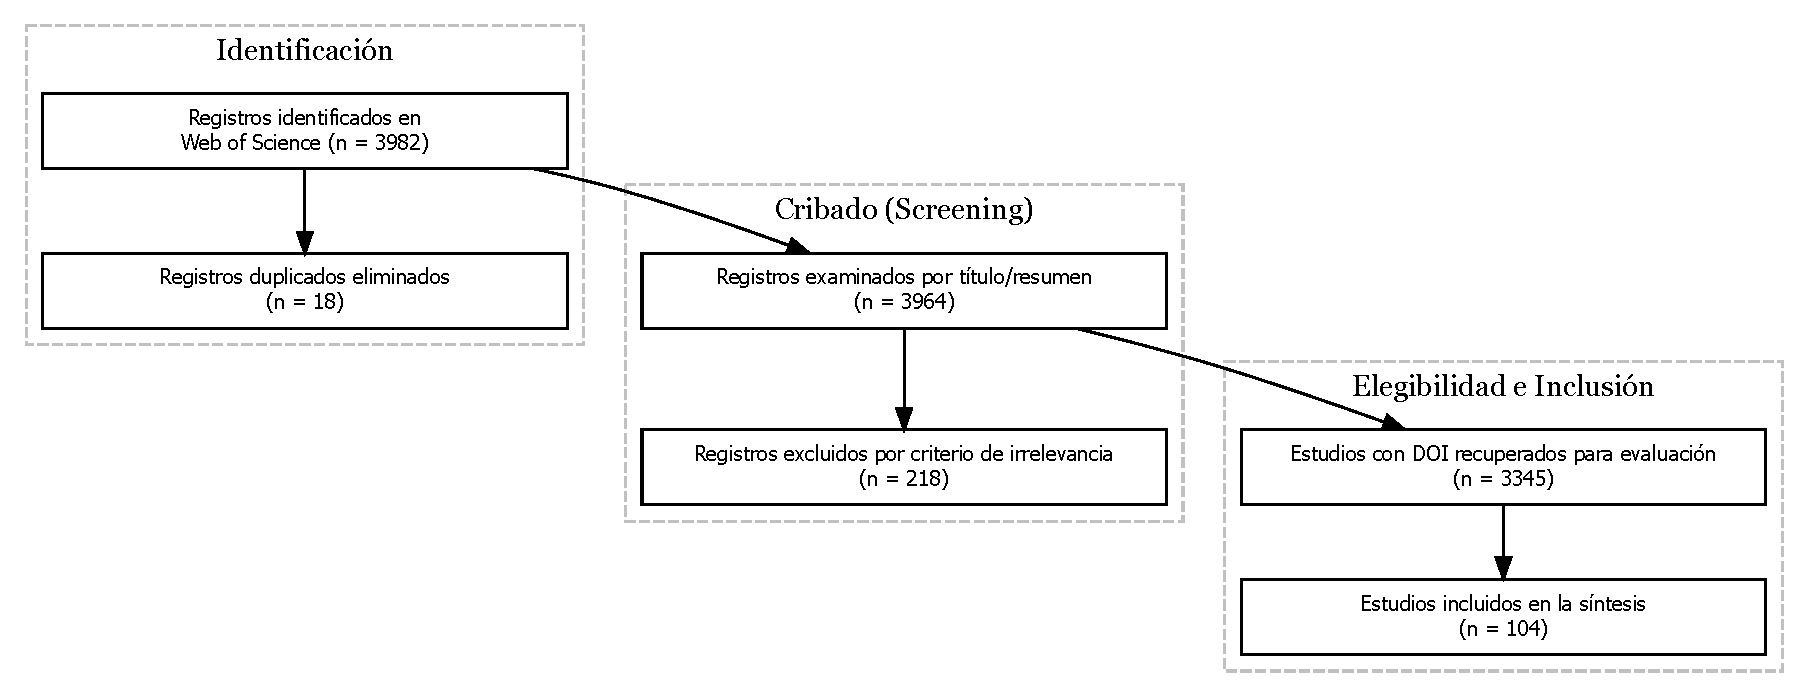
\includegraphics[width=1.0\textwidth]{../images/prisma-flowchart.pdf}
    \caption{Diagrama de Flujo Metodológico PRISMA 2020 para la selección de bibliografía de WoS.}
    \label{fig:prisma-flowchart}
\end{figure}
% \section{Anexo 2: Fotos y Material Visual de Apoyo}

A continuación, se presentan las imágenes y el material visual de apoyo utilizado en el desarrollo de la investigación. Con respecto a las imágenes, se incluyen capturas de pantalla de los resultados de las búsquedas en bases de datos y repositorios, así como gráficos y tablas que ilustran los hallazgos clave. Este material visual complementa la información presentada en el Anexo 1 y proporciona evidencia adicional sobre la metodología y los resultados obtenidos.

\subsection{Justificación Fotos y Material Visual}
La selección de \textit{Fotos y Material Visual} responde a la necesidad de documentar de manera visual los procesos de búsqueda y análisis de la literatura especializada. Las imágenes permiten una comprensión más clara de los pasos seguidos en la estrategia híbrida de revisión bibliográfica, así como de los resultados obtenidos en términos de cobertura geográfica, temporal y temática. Además, el material visual facilita la replicabilidad del estudio y la verificación de los hallazgos por parte de otros investigadores interesados en el bienestar socioeconómico en la región del Cono Sur.


% Lista de referencias bibliográficas
\printbibliography
\end{document}